\documentclass[conference]{IEEEtran}
\IEEEoverridecommandlockouts
% The preceding line is only needed to identify funding in the first footnote. If that is unneeded, please comment it out.
\usepackage{cite}
\usepackage{amsmath,amssymb,amsfonts}
\usepackage{algorithmic}
\usepackage{graphicx}
\usepackage{textcomp}
\usepackage{xcolor}
\usepackage{array}
\def\BibTeX{{\rm B\kern-.05em{\sc i\kern-.025em b}\kern-.08em
    T\kern-.1667em\lower.7ex\hbox{E}\kern-.125emX}}
\begin{document}

\title{Explainable Artificial Intelligence \\ {Methodology for Handwritten Applications}}

\author{\IEEEauthorblockN{Paul Whitten, Francis Wolff, Chris Papachristou}
\IEEEauthorblockA{\textit{Electrical, Computer, and Systems Engineering} \\
\textit{Case School of Engineering} \\
\textit{Case Western Reserve University} \\
Cleveland, OH, USA \\
pcw@case.edu, fxw12@case.edu, cap2@case.edu}

}

\maketitle

\begin{abstract}
There has been explosive growth of practical AI in recent years.
%However, inferential results of AI systems are not readily explainable to humans.
A major concern of current AI systems is an inability to explain inferential decisions.
%Explainable artificial intelligence has been posed to mitigate these concerns.
This work explores an Explainable Artificial Intelligence (XAI) methodology that provides explanations
for classification decisions.  Experimental results using the MNIST handwritten digit database are provided with explainable conclusions.
\end{abstract}

\begin{IEEEkeywords}
explainable, artificial intelligence, machine learning
\end{IEEEkeywords}

\section{Introduction}

Recent advances in Machine Learning (ML) have brought about wide adoption of ML algorithms for many applications.  Despite various successes, there is a reluctance to adopt ML in some applications because ML behaves like a black box.  Decision-making by the black box is often not explainable to humans. 

EU regulations, GDPR \cite{gdpr2016} Article 13 (2)(f), indicates a controller shall provide a data subject with meaningful information about the logic involved in automated decision making or profiling.  Other countries are considering API legislation, especially the US\cite{burt_2021}. There is debate over the right to an explanation when using AI in significant decisions\cite{selbst}.  The motivation for this work is the need for explainability in AI.

%\begin{figure}[htbp]
%\centerline{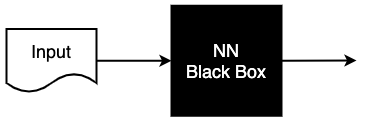
\includegraphics[width=40mm]{./images/unexplainable.png}}
%\caption{An unexplainable NN.}
%\label{unexplainable}
%\end{figure}

%\begin{figure}[htbp]
%\centerline{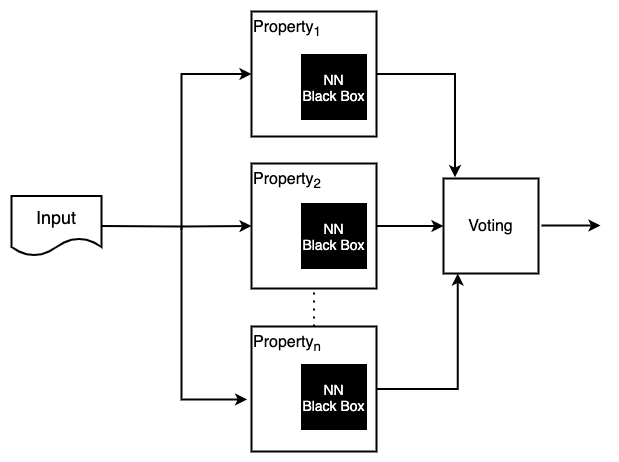
\includegraphics[width=95mm]{./images/explainable.png}}
%\caption{Fine grained explainable NN classification based on properties.}
%\label{explainable}
%\end{figure}

This work approaches the widely studied problem of classifying images of handwritten digits into the ten decimal digit classes from an XAI perspective.  Our goal is to provide explainable classification in the form of rationale that a layperson can understand.  This is achieved using an explainable architecture, with fine-grained classification decisions based on explainable properties, and a methodology for constructing the explainable architecture.  We do not attempt to explain the internal structure of the ML model.  In this work ML models still act as black boxes, but through finer-grained classification, we add an element of explainability.

Using the MNIST\cite{deng2012mnist} handwritten digit database, we apply the methodology and architecture.  The approach is outlined herein, along with test cases and examples of explainability.  Finally, we present results and metrics to gauge accuracy and explainability.

We aim to pose a means of explaining classification to a human.  We do not wish to compete with established algorithms that perform exceptionally well in classification of input \cite{keysers07} \cite{lecun98} \cite{schm2012}.  The effort required to apply the methodology in this work is significant compared to training a classifier that will act as a black box and, therefore, not explainable.

While we approach XAI for a specific classification problem, in the MNIST handwritten digit database, the methodology translates to other challenges requiring explainable classification among a finite set of classes.

\section{Related work}

The ability to map the learning classifier or recognizer to human-based explainability is a challenging task for human understandability.  Currently, there are at least seventeen explainable techniques such as
decision tree-based, rule-based (i.e. knowledgebase), salience mapping,
sensitivity-based analysis, feature importance, fuzzy-based, neural-network, and generic-programming based.  These techniques use one of three basic evaluation approaches: application-grounded, human-grounded and functionally grounded. \cite{BlackBox18} \cite{Arrieta2020ExplainableAI} \cite{Survey18} \cite{Fuzzy19} \cite{Hagras18}  \cite{GP18}

Distributed and fault tolerant systems research has provided several examples of voting \cite{avizienis} and probabilistic models for the voting problem \cite{blough}.

\section{Overview}

 \begin{figure}[htbp]
\centerline{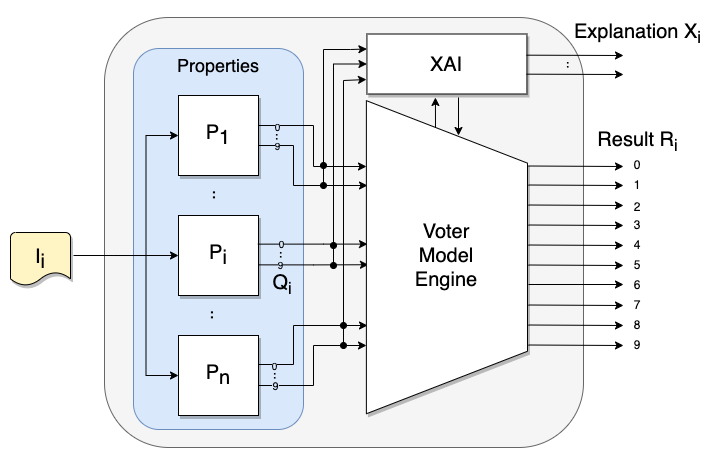
\includegraphics[width=90mm]{./images/voting_prop_nn_2.png}}
\caption{XAI Architecture}
\label{voting}
\end{figure}

Explainable properties and related input transformations are the basis for the explainable methodology.  The architecture performs distinct classification decisions for each property transformation.  Those distinct classifications are input to a voter to provide a final classification decision.  Explainability comes from relating the fine-grained decisions for property transformations to compose rationale for a user.

Fig.~\ref{voting} depicts the explainable architecture used in this work.  $I_i$ represents the $i$th input to the architecture.  The architecture consists of Properties, a Voter Model Engine (VME),  and an Explainable Artificial Intelligence block.   Explainable properties are defined as descriptive qualities of a sample input that mean something to a user in the problem domain, especially to justify a classification decision.   Explainable properties $P_1$ through $P_n$ are outlined in the blue Property rectangle.  Each property represents logic for a classification based solely on the property.   $Q_j$ represents the $j$th property's classification output.

The VME relies on classifications from the explainable properties, $Q_j$, and feedback from the XAI block to make a final classification decision.   We explore two voting model schemes detailed in Section \ref{subsection:Voting}.

The XAI block, in Fig.~\ref{voting}, consists of a knowledgebase and logic to generate an explanation for the user.  Inputs to the XAI block are explainable property classifications, $Q_j$, and the VME decision.  The XAI knowledgebase contains information on explainable properties, training results, and metrics related to the effectiveness of properties.  The explanation provided by the XAI block consists of rationale that relates to the explainable properties contributing to the classification decision.

 \begin{figure}[htbp]
\centerline{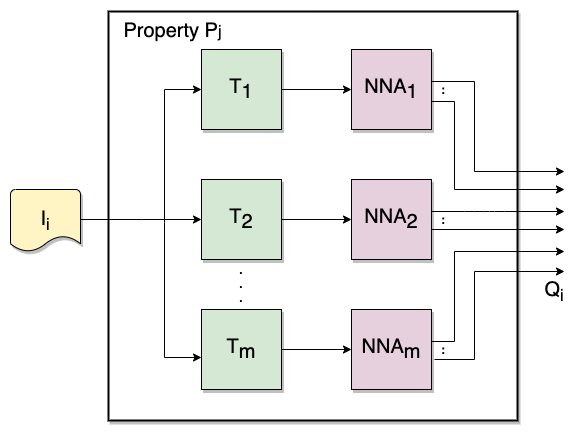
\includegraphics[width=90mm]{./images/property_transforms.png}}
\caption{Architecture of a single property for multiple transformations.}
\label{proptrans}
\end{figure} 

A property transformation is a modifying function applied to the input.  Transformations identify the explainable property in the input.  Each property may have one or more transformations.   Fig.~\ref{proptrans} represents transformations in the explainable architecture.  The outer square represents the $j$th property from Fig.~\ref{voting}.  The boxes labeled $T_1$ through $T_m$ indicate $m$ transformations of the input related to property $j$.  Transformed input is fed to a trained Neural Network Architecture (NNA) to make classification decisions.  Classification output then flows to the VME as shown in Fig.~\ref{voting}.

\section{Methodology}
 
Our methodology for achieving explainable ML classification involves the following steps:
%\begin{itemize}
%\item Discover explainable properties.
%\item Define transformations for explainable properties.
%\item Transform training data.
%\item Produce trained explainable property-specific NNAs.
%\item Build a Knowledgebase across the explainable properties.
%\item Devise a voting scheme.
%\item Use a test dataset to provide feedback.
%\end{itemize}

\subsubsection{Discover Explainable Properties}
An explainable property is an attribute of a sample in the problem domain that may differentiate classes and provide a rationale for a classification decision to a user.   An explainable property need not be present in all classes.  Discovering explainable properties may require manual analysis of sample inputs.

\subsubsection{Define and Implement Transformations}
Data transformations are next defined and implemented to highlight explainable properties in the input.  Transforms may be known algorithms of feature detection and extraction that relate to explainable properties.

\subsubsection{Transform Training Data} 
We next generate a transformed training dataset by submitting all elements from the training set to the property transformations.  The output from property transformations is stored for later use in training the property transform specific NNAs. 

\subsubsection{Produce Trained Property NNAs}
The next step involves initializing unique NNAs for each property transformation.  The NNAs are trained, using supervised ML techniques, from the data stored from the previous step.  The result is a set of trained NNAs that produce classifications for the explainable property transforms.

\subsubsection{Build an XAI Knowledgebase}
After training, we process the training set again and populate the XAI knowledgebase with the property classification results.  The knowledgebase also stores explainable property descriptions and each property's classification result for training data.  Metrics on the per-class effectiveness of explainable properties are calculated and stored in the knowledgebase for use by the VME.

\subsubsection{Devise a Voting Scheme}
We next devise a voting scheme in the VME.  The purpose of the voting scheme is to select among the potentially conflicting votes from the explainable property transformation classifications.  Information from the knowledgebase and explainable property classifications are input for voting decisions.  We discuss probabilistic and ML based voting schemes later in Section \ref{subsection:Voting}.

\subsubsection{Provide User Feedback}
Finally, when we present test data to the architecture, we evaluate the results and determine if they are sufficient.  The performance of the explainable property transforms for particular classes are examined for effectiveness.  We identify classes with poor results and seek new properties.  We eliminate ineffective properties or transforms.

\section{Approach}

This section presents the approach of applying the methodology to the MNIST handwritten digit database. 

\subsection{Explainable Properties}

Through a manual review of samples in MNIST, we identified explainable properties related to shapes and characteristics of the digits.  The explainable properties we identified and utilized are listed in the Property column of Table~\ref{transsample}.

\subsection{Transformations}
 
Digital image processing techniques that relate to and highlight the explainable properties were used as transforms.  The Transform column in Table~\ref{transsample} lists transformations for the various properties.  The figure also shows example MNIST digits, $I_i$, and their resulting transformed images, $T_j(I_i)$.

\bgroup
\renewcommand{\arraystretch}{1.8}
%\setlength\tabcolsep{2mm}
\begin{table}
\caption{Properties and transforms for the MNIST example}
\centering
\resizebox{\columnwidth}{!}{%
\begin{tabular}{ c | p{0.23\linewidth} | p{0.23\linewidth} | ccc | }
\cline{2-6}
$P_j$ & Property & Transform & $I_i$ &  &  $T_j(I_i)$ \\
\hline \hline
$P_1$ & Stroke & Skeleton & \raisebox{-.5\height}{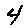
\includegraphics[width=6mm]{./digit-images/4-11.png}} & $\rightarrow$ & \raisebox{-.5\height}{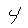
\includegraphics[width=6mm]{./digit-images/4-11-skel.png}} \\
\hline
$P_2$ & Circle & Hough Circle & \raisebox{-.5\height}{
\includegraphics[width=6mm]{./digit-images/6-17.png}} & $\rightarrow$ & \raisebox{-.5\height}{
\includegraphics[width=6mm]{./digit-images/6-17-circle.png}} \\
\hline
$P_3$ & Crossings & Crossings & \raisebox{-.5\height}{
\includegraphics[width=6mm]{./digit-images/4-2.png}} & $\rightarrow$ & \raisebox{-.5\height}{
\includegraphics[width=6mm]{./digit-images/4-2-crossing.png}} \\
\hline
$P_4$ & Circle & Hough Ellipse & \raisebox{-.5\height}{
\includegraphics[width=6mm]{./digit-images/0-3.png}} & $\rightarrow$ & \raisebox{-.5\height}{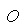
\includegraphics[width=6mm]{./digit-images/0-3-ellipse.png}} \\
\hline
$P_5$ & Circle & Multiple Ellipse Circle & \raisebox{-.5\height}{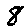
\includegraphics[width=6mm]{./digit-images/8-4.png}} & $\rightarrow$ & \raisebox{-.5\height}{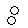
\includegraphics[width=6mm]{./digit-images/8-4-ellipse-circle.png}} \\
\hline
$P_6$ & Endpoints & Endpoints & \raisebox{-.5\height}{
\includegraphics[width=6mm]{./digit-images/2-2.png}} & $\rightarrow$ & \raisebox{-.5\height}{
\includegraphics[width=6mm]{./digit-images/2-2-endpoint.png}} \\
\hline
$P_7$ & Enclosed Region & Flood Fill & \raisebox{-.5\height}{
\includegraphics[width=6mm]{./digit-images/0-2.png}} & $\rightarrow$ & \raisebox{-.5\height}{
\includegraphics[width=6mm]{./digit-images/0-2-fill.png}} \\
\hline
$P_8$ & Line & Hough Line & \raisebox{-.5\height}{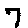
\includegraphics[width=6mm]{./digit-images/7-20.png}} & $\rightarrow$ & \raisebox{-.5\height}{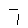
\includegraphics[width=6mm]{./digit-images/7-20-line.png}} \\
\hline
$P_9$ & Enclosed Region & Skeleton Flood Fill & \raisebox{-.5\height}{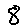
\includegraphics[width=6mm]{./digit-images/8-3.png}} & $\rightarrow$ & \raisebox{-.5\height}{
\includegraphics[width=6mm]{./digit-images/8-3-skel-fill.png}} \\
\hline
\end{tabular}%
}
\centering
\label{transsample}
\end{table}
\egroup

The Stroke property is meant to represent the minimal path of the writing implement to trace the digit.  The morphological skeleton transformation is a one-pixel connected representation of the digit,  representing the stroke.  We utilized the Lee\cite{Lee1994} algorithm for the skeleton.
$P_2$, $P_4$, and $P_5$ are the circle property with corresponding transforms $T_2$, $T_4$, and $T_5$ representing the Hough Circle, the Hough Ellipse, and multiple non-overlapping circles and ellipses.
$P_3$ and $T_3$ are the crossings property and transform representing the intersection of line segments in a digit.  $T_3$ involves taking the skeleton and then finding activated pixels with more than two neighbors.   The endpoints property and transform, $P_6$ and $T_6$, involved taking activated pixels in the skeleton with only one neighbor.
Property $P_7$ and $P_9$ for enclosed regions used transform $T_7$ which involved a flood fill and $T_9$ the flood fill of the skeleton.  The line property and transform, $P_8$ and $T_8$, uses an algorithm to find the non-overlapping Hough Lines.

\subsection{Transforming Training Data}

The various transforms were applied to the MNIST data using implementations in the Python scikit-image\cite{scikitimage} library version 0.17.2.  The resulting transformed images were stored in MNIST IDX files for each property transform.

\subsection{Training}

The trained NNAs were implemented using the Python scikit-learn\cite{scikitlearn} version 0.23.2 Multi-Layer Perceptrons.  The property transform NNAs were trained using the transformed data stored in the MNIST IDX files.

\subsection{Knowledgebase}

After training the NNAs, the transformed training data was presented to the NNAs and results were stored in a data structure that was serialized as JSON.  The JSON was loaded to in-memory maps for performing metric calculation and efficient runtime access.  Textual property labels and descriptions were also stored in the knowledgebase for composing explainable rationale in the XAI block.

\subsection{Voting Schemes}
\label{subsection:Voting}

The first voting scheme we present is probabilistic.  In this scheme, we use the knowledgebase to identify each explainable property transformation's effectiveness to correctly predict a digit.   The effectiveness for an explainable property transformation, $j$, to select a particular digit, $d$,  is given by:
\begin{equation}\label{effectiveness}
E_{j,d}  = \frac{|A|}{|B|}
\end{equation}
where $A$ is the set of correct classifications of explainable property transformation $j$ of the digit $d$ and $B$ is the set of elements of digit $d$.  The weight of the effectiveness for each digit, $d$, is:
\begin{equation}\label{weight}
W_d=\sum_j E_{j, d}
\end{equation}
The confidence for the digit $d$ is calculated by the VME and is given by:
\begin{equation}\label{conf}
C_d=\frac{W_d}{\sum\limits_kW_k}
\end{equation}
The denominator is the sum of all weights for classes that were selected by a property.  If multiple digits are selected by the properties, the digit with the highest confidence will be chosen by the VME.

The second voting scheme was NN based.  We utilized explainable property transformation output and labels from MNIST, stored in the knowledgebase, to train a Multi-Layer Perceptron model in the NN VME.

\subsection{ User Feedback}

When evaluating early results, there was particular difficulty with the circle transforms for some digits.   The single circle transforms worked well for detecting digits six and nine but performed rather poorly for eight and zero.  The ellipse proved better in extracting characteristics of handwritten zeros.   Adding a transform that used multiple non-overlapping circles or ellipses was also an improvement for the digit eight.  We experimented with the inflection point property, and corner detection transforms, but the classification results were poor for all digit classes, so the property was eliminated.

\section{Examples}

Detailed examples from MNIST follow in this section by first providing aggregate property classification results for the digits five and six and then explainable results from three different input images.

Tables ~\ref{table:digit5out} and ~\ref{table:digit6out} show the property transformation NNA output and statistics for properties for digits five and six.  The tables represent the results from reprocessing all of the training digits labeled five and six.  Columns two through ten of the tables represent the property transformations, $P_j$ from Table~\ref{transsample}.  The first row of the tables represents effectiveness, $E_{j,d}$, where $j$ is the property transform, and $d$ is the digit.  The second, third, and fourth rows represent the standard deviation, kurtosis, and skew of the digit outputs for each property.  The numbered rows in the tables represent the means of the property outputs for each digit.  The last two rows are the false-positive and false-negative rates.

We observe that the Stroke property, $P_0$, performed very well in both digits.  The next highest performing property in both tables was the endpoint property, $P_6$, with 0.85 and 0.93 effectiveness.  The digit six also had good classification results for the enclosed region properties, $P_7$ and $P_9$.  The digit six also performed better than the five in the properties related to the circle, $P_2$, $P_4$, and $P_5$.  The digit five had among the poorest performance as observed from the relatively low percent correct and high false-negative rates.

\begin{table}
\caption{Digit 5 Outputs}
\centering
\resizebox{\columnwidth}{!}{%
\begin{tabular}{ | c ||  c | c | c | c | c | c | c | c | c |}
Digit 5 & $P_1$ & $P_2$ & $P_3$ & $P_4$ & $P_5$ & $P_6$ & $P_7$ & $P_8$ & $P_9$ \\
\hline \hline
$E_{j,5}$  & 1.00 & 0.14 & 0.57 & 0.21 & 0.22 & 0.85 & 0.04 & 0.70 & 0.06 \\
\hline
$\sigma$ & 0.30& 0.08& 0.08& 0.07& 0.09& 0.25& 0.07& 0.21& 0.08 \\
\hline
k & 10.0& 4.00& -1.86& 5.56& 6.23& 9.55& -1.94& 9.78& -2.06 \\
\hline
skew & 3.16& 1.91& 0.33& 2.32& 2.41& 3.07& -0.03& 3.12& 0.06 \\
\hline
0 & 0.00 & 0.12 & 0.21 & 0.09 & 0.07 & 0.00 & 0.01 & 0.02 & 0.02 \\
\hline
1 & 0.00 & 0.05 & 0.22 & 0.06 & 0.04 & 0.11 & 0.19 & 0.01 & 0.18 \\
\hline
2 & 0.00 & 0.05 & 0.05 & 0.06 & 0.05 & 0.00 & 0.09 & 0.03 & 0.07 \\
\hline
3 & 0.00 & 0.16 & 0.08 & 0.15 & 0.15 & 0.00 & 0.15 & 0.08 & 0.18 \\
\hline
4 & 0.00 & 0.05 & 0.01 & 0.06 & 0.05 & 0.00 & 0.12 & 0.02 & 0.13 \\
\hline
5 & 1.00 & 0.30 & 0.20 & 0.28 & 0.35 & 0.85 & 0.19 & 0.73 & 0.19 \\
\hline
6 & 0.00 & 0.10 & 0.07 & 0.06 & 0.09 & 0.01 & 0.03 & 0.04 & 0.04 \\
\hline
7 & 0.00 & 0.05 & 0.17 & 0.07 & 0.04 & 0.00 & 0.19 & 0.01 & 0.21 \\
\hline
8 & 0.00 & 0.11 & 0.02 & 0.09 & 0.10 & 0.01 & 0.01 & 0.04 & 0.01 \\
\hline
9 & 0.00 & 0.04 & 0.02 & 0.07 & 0.04 & 0.01 & 0.03 & 0.03 & 0.03 \\
\hline
false pos. \%  & 0.0 & 0.5 & 0.2 & 0.4 & 0.7 & 0.4 & 0.0 & 0.3 & 0.0 \\
\hline
false neg. \%  & 0.0 & 84.8 & 94.1 & 78.8 & 78.3 & 13.4 & 96.2 & 29.2 & 94.5 \\
\hline
\end{tabular}%
}
\label{table:digit5out}
\end{table}

\begin{table}
\caption{Digit 6 Outputs}
\centering
\resizebox{\columnwidth}{!}{%
\begin{tabular}{ | c ||  c | c | c | c | c | c | c | c | c |}
Digit 6 & $P_1$ & $P_2$ & $P_3$ & $P_4$ & $P_5$ & $P_6$ & $P_7$ & $P_8$ & $P_9$ \\
\hline \hline
$E_{i,6}$  & 1.00 & 0.47 & 0.50 & 0.32 & 0.49 & 0.93 & 0.82 & 0.71 & 0.83 \\
\hline
$\sigma$ & 0.30& 0.11& 0.13& 0.09& 0.13& 0.26& 0.24& 0.21& 0.25 \\
\hline
k & 10.0& 8.51& 8.62& 9.86& 9.47& 9.96& 9.94& 9.89& 9.93 \\
\hline
skew & 3.16& 2.84& 2.89& 3.13& 3.05& 3.15& 3.15& 3.14& 3.15 \\
\hline
0 & 0.00 & 0.10 & 0.04 & 0.07 & 0.08 & 0.02 & 0.00 & 0.03 & 0.00 \\
\hline
1 & 0.00 & 0.05 & 0.05 & 0.07 & 0.05 & 0.01 & 0.04 & 0.01 & 0.03 \\
\hline
2 & 0.00 & 0.06 & 0.14 & 0.06 & 0.06 & 0.02 & 0.02 & 0.03 & 0.01 \\
\hline
3 & 0.00 & 0.10 & 0.05 & 0.07 & 0.08 & 0.00 & 0.03 & 0.05 & 0.03 \\
\hline
4 & 0.00 & 0.03 & 0.04 & 0.07 & 0.04 & 0.00 & 0.03 & 0.05 & 0.02 \\
\hline
5 & 0.00 & 0.10 & 0.07 & 0.05 & 0.09 & 0.01 & 0.03 & 0.03 & 0.02 \\
\hline
6 & 1.00 & 0.43 & 0.49 & 0.38 & 0.50 & 0.89 & 0.82 & 0.73 & 0.84 \\
\hline
7 & 0.00 & 0.06 & 0.05 & 0.08 & 0.05 & 0.00 & 0.03 & 0.01 & 0.04 \\
\hline
8 & 0.00 & 0.03 & 0.09 & 0.07 & 0.03 & 0.03 & 0.00 & 0.04 & 0.00 \\
\hline
9 & 0.00 & 0.03 & 0.03 & 0.08 & 0.04 & 0.00 & 0.01 & 0.03 & 0.01 \\
\hline
false pos. \%  & 0.0 & 2.6 & 2.5 & 0.5 & 2.2 & 0.7 & 0.2 & 0.6 & 0.0 \\
\hline
false neg. \%  & 0.0 & 53.3 & 50.1 & 67.5 & 50.7 & 6.6 & 18.1 & 28.1 & 16.8 \\
\hline
\end{tabular}%
}
\label{table:digit6out}
\end{table}

Mean digit values from the Property NNAs are also represented  in Fig.~\ref{digit5votes} and ~\ref{digit6votes} as three dimensional surface plots for digits five and  and six.

\begin{figure}[htbp]
\begin{minipage}{0.48\textwidth}
\centerline{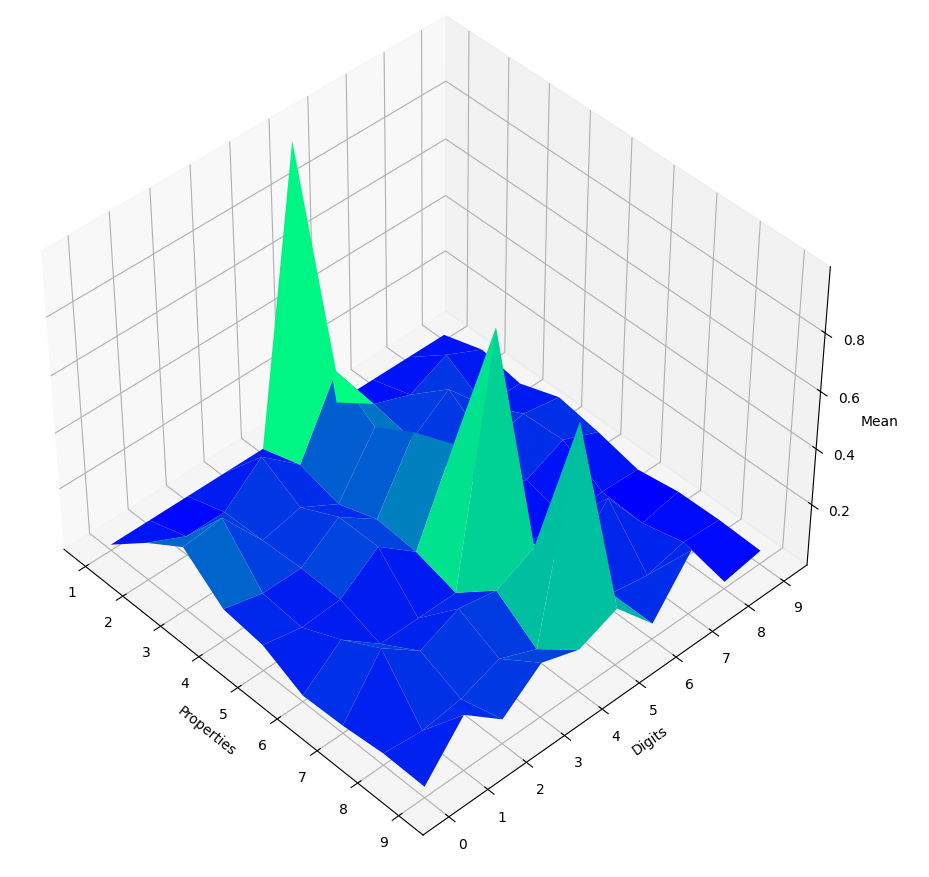
\includegraphics[width=60mm]{./images/digit-5.png}}
\caption{Property output for digit 5}
\label{digit5votes}
\end{minipage}
\begin{minipage}{0.48\textwidth}
\centerline{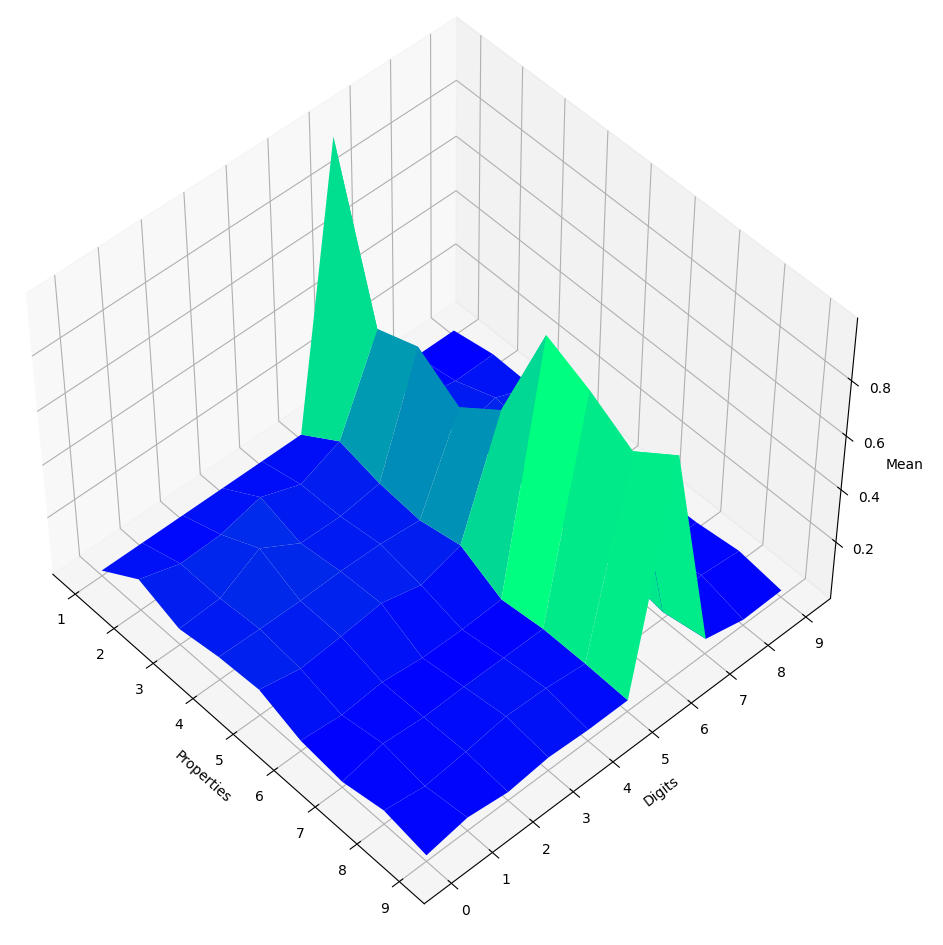
\includegraphics[width=60mm]{./images/digit-6.png}}
\caption{Property output for digit 6}
\label{digit6votes}
\end{minipage}
\end{figure}

%\begin{table}[htbp]
%\caption{Properties, Transforms and Property Identifiers}
%\centering
%\begin{tabular}{| c | c | c |}
%\hline
% Identifier & Explainable Property & Transform \\
%\hline\hline
%$P_1$ & Stroke & Skeleton \\
%\hline
%$P_x$ & Circle & Hough Circle \\
%\hline
%$P_x$ & Crossings & Crossing Point \\
%\hline
%$P_x$ & Ellipse & Hough Ellipse \\
%\hline
%$P_x$ & Ellipse + Circle & Hough Ellipse and Circle \\
%\hline
%$P_x$ & Endpoints & Endpoints \\
%\hline
%$P_x$ & Enclosed Region & Flood Fill \\
%\hline
%$P_x$ & Line & Hough Line \\
%\hline
%$P_x$ & Enclosed Region of Skeleton & Skeleton Flood Fill \\
%\hline
%\end{tabular}
%\label{table:tblproptrans}
%\end{table}

%\begin{figure}[htbp]
%\centerline{
\includegraphics[width=15mm]{./digit-images/5-0.png}}
%\caption{Example 1 of a handwritten digit five}
%\label{example1}
%\end{figure}

 \begin{figure}[htbp]
 \begin{minipage}{0.15\textwidth}
\centerline{
\includegraphics[width=15mm]{./digit-images/5-0.png}}
\caption{Example 1}
\label{example1}
\end{minipage}
 \begin{minipage}{0.15\textwidth}
\centerline{
\includegraphics[width=15mm]{./digit-images/9-9.png}}
\caption{Example 2}
\label{example2}
\end{minipage}
\begin{minipage}{0.15\textwidth}
 \centerline{
\includegraphics[width=15mm]{./digit-images/2-4.png}}
\caption{Example 3}
\label{example3}
\end{minipage}
\end{figure}

Next, we present three interesting MNIST digits and review the property classifications, effectiveness,  confidence, and explainability.  Stepping through the procedures of the probabilistic voting scheme, we show the classification results for the digits as well as the explainability rationale from XAI.

\begin{table}[htbp]
\caption{Prob. voting, effectiveness, and explainability for ex. 1}
\centering
\begin{tabular}{| c | c | c | c | c | p{0.08\linewidth} | p{0.08\linewidth} |}
\cline{4-7}
\multicolumn{3}{c}{} & \multicolumn{2}{|c|}{Effectiveness} & \multicolumn{2}{c|}{Explainability} \\
\hline
 $P_j$ & Property & Vote & $E_{j,5}$ & $E_{j,6}$ & $X_5$ & $X_6$ \\
\hline \cline{0-6}
$P_1$ & Stroke & 5 & 1.00 &  & \checkmark &  \\ 
\hline
$P_2$ & Circle & 6 &  & 0.47 &  & \checkmark \\
\hline
$P_3$ & Crossing &  &  &   &  &  \\
\hline
$P_4$ & Circle &  &  &  &  &  \\
\hline
$P_5$ & Circle & 6 &  & 0.49 &  & \checkmark \\
\hline
$P_6$ & Endpoint & 5 & 0.85 &  & \checkmark &  \\
\hline
$P_7$ & Encl. Reg. &  &  &  &  &  \\
\hline
$P_8$ & Line & 5 & 0.70 &  & \checkmark &  \\
\hline
$P_9$& Encl. Reg. &  &  &  &  &  \\
\hline \cline{0-6}
\multicolumn{3}{|c|}{Weight Totals} & $2.55$ & $0.96$ & \multicolumn{2}{c|}{$\sum W_k=3.51$} \\
\cline{0-6}
\multicolumn{3}{|c|}{Confidence} & $72.6\%$ & $27.4\%$ & \multicolumn{2}{c}{} \\
\cline{0-4}
\end{tabular}
\label{table:example1}
\end{table}

\begin{table}[htbp]
\caption{Rationale for example 1}
\centering
\begin{tabular}{| p{0.04\linewidth} | p{0.14\linewidth} | p{0.65\linewidth} |}
\hline
 $X_d$ & Confidence & Explainable Description \\
\hline \cline{1-3}
$X_5$ & 72.6\% & Confidence is high for interpreting this digit as a five due to the stroke, endpoint, and line properties. \\ 
\hline
$X_6$ & 27.4\% & Confidence is low for interpreting this digit as a six due to circle properties. \\
\hline
\end{tabular}
\label{table:exexample1}
\end{table}

The first example digit, labeled a five, is shown in Fig.~\ref{example1}.  Voting and explainability is detailed in Table ~\ref{table:example1}.  The property votes for this example are shown in the Vote column.  Empty cells are properties that did not have a sufficiently strong opinion on a particular digit.  I.e., no digit was above a threshold for that property.   The $E_{j,d}$ columns give the effectiveness of a property $j$ to correctly select digit $d$.  The effectiveness values are from the knowledgebase using Eq. (\ref{effectiveness}).   The stroke $(P_1)$, endpoint $(P_6)$, and line $(P_8)$ properties suggest the digit is a five with effectiveness $E_{1,5}= 1.00$, $E_{6,5}=0.85$, and $E_{8,5}=0.70$.  The weight of effectiveness for the digit five is $W_5=2.55$, given by Eq. (\ref{weight}).  The circle $(P_2)$ and $(P_5)$ properties suggest that the digit is a six with effectiveness $E_{2,6}=0.47$ and $E_{5,6}=0.49$  and a weight of $W_6=0.96$.  Taking the sum of all weights, $\sum\limits_k W_k=3.51$.  Confidence, as given by Eq. (\ref{conf}), for the five, is given as $C_5=\frac{2.55}{3.51} = 72.6\%$.  Alternatively, six was suggested by properties where confidence is $C_6=\frac{0.96}{3.51}=27.4\%$.  Five wins because $C_6=27.4\% < 72.6\%=C_5$.  We also observe that the explainability, $X_d$, columns provide the rationale for each of the digits that was selected.  The logic in the XAI block references property information from explainability columns as well as the confidence from the VME and assembled as shown in Table~ \ref{table:exexample1}.   Rationale defending the decision is presented to the user indicating, confidence is high for interpreting this digit as a five due to the stroke, endpoint, and line properties. 

%\begin{figure}[htbp]
%\centerline{
\includegraphics[width=15mm]{./digit-images/9-9.png}}
%\caption{Example 2 of a handwritten digit nine}
%\label{example2}
%\end{figure}

%\begin{table}[htbp]
%\caption{Property Votes for Example 2}
%\centering
%\begin{tabular}{| c | c | c |}
%\hline
% Property Id & Vote & Weight \\
%\hline\hline
%$P_0$ & 9 & 1.000 \\ 
%\hline
%$P_1$ & 3 & 0.327 \\
%\hline
%$P_2$ & 5 & 0.057 \\
%\hline
%$P_3$ & - & - \\
%\hline
%$P_4$ & - & - \\
%\hline
%$P_5$ & 6 & 0.932 \\
%\hline
%$P_6$ & 9 & 0.809 \\
%\hline
%$P_7$ & - & - \\
%\hline
%$P_8$ & 9 & 0.821 \\
%\hline
%\end{tabular}
%\label{table:example2}
%\end{table}

The second example,  labeled a nine, is shown in Fig.~\ref{example2}.  Table ~\ref{table:example2} shows the property predictions, voting results, and explainability.  In this example three properties selected the digit nine and three other properties selected the digits three, five, and six.  The results from the VME for this example were that nine was selected with a $66.5\%$ confidence and an explanation from Table~\ref{table:exexample2} explain that confidence is high for interpreting this digit as a nine due to the stroke and enclosed region properties.  We noted on this example that it is surprising that none of the properties indicated an eight because of the example's similarity to a digit eight.  

\begin{table}[htbp]
\caption{Prob. voting, effectiveness, and explainability for ex. 2}
\centering
\resizebox{\columnwidth}{!}{%
\begin{tabular}{| c | c | c | c | c | c | c | c | c | c | c |}
\cline{4-11}
\multicolumn{3}{c}{} & \multicolumn{4}{|c|}{Effectiveness} & \multicolumn{4}{c|}{Explainability} \\
\hline
 $P_j$ & Property & Vote & $E_{j,3}$ & $E_{j,5}$ & $E_{j,6}$ & $E_{j,9}$ & $X_3$ & $X_5$ & $X_6$ & $X_9$ \\
\hline \cline{0-10}
$P_1$ & Stoke & 9 &  &  &  & 1.00 &  &  &  & \checkmark \\ 
\hline
$P_2$ & Circle & 3 & 0.33 &  &  &  & \checkmark &  &  &  \\
\hline
$P_3$ & Crossing & 5 &  &  0.06 &  &  &  & \checkmark &  &  \\
\hline
$P_4$ & Circle &  &  &  &  &  &  &  &  &  \\
\hline
$P_5$ & Circle &  &  &  &  &  &  &  &  &  \\
\hline
$P_6$ & Endpoint & 6 &  &  & 0.93 &  &  &  & \checkmark &  \\
\hline
$P_7$ & Encl. Reg. & 9 &  &  &  & 0.81 &  &  &  & \checkmark \\
\hline
$P_8$ & Line &  &  &  &  &  &  &  &  &  \\
\hline
$P_9$ & Encl. Reg. & 9 &  &  &  & 0.82 &  &  &  & \checkmark \\
\hline \cline{0-10}
\multicolumn{3}{|c|}{Weight} & 0.33 & 0.06 & 0.93 & 2.63 & \multicolumn{4}{c|}{$\sum W_k=3.95$} \\
\cline{0-10}
\multicolumn{3}{|c|}{Confidence} & $8.3\%$ & $1.7\%$ & $23.5\%$ & $66.5\%$ & \multicolumn{4}{c}{} \\
\cline{0-6}
\end{tabular}%
}
\label{table:example2}
\end{table}

\begin{table}[htbp]
\caption{Rationale for example 2}
\centering
\begin{tabular}{| p{0.04\linewidth} | p{0.14\linewidth} | p{0.65\linewidth} |}
\hline
 $X_d$ & Confidence & Explainable Description \\
\hline \cline{1-3}
$X_9$ & 66.5\% & Confidence is high for interpreting this digit as a nine due to the stroke and enclosed region properties. \\
\hline
$X_6$ & 23.5\% & Confidence is low for interpreting this digit as a six due to the endpoint property.  \\
\hline
$X_3$ & 8.3\% & Confidence is low for interpreting this digit as a three due to the circle circle property.  \\ 
\hline
$X_5$ & 1.7\% & Confidence is almost zero for interpreting this digit as a five due to the crossing property. \\
\hline
\end{tabular}
\label{table:exexample2}
\end{table}

%\begin{figure}[htbp]
%\centerline{
\includegraphics[width=15mm]{./digit-images/2-4.png}}
%\caption{Example 3 of a handwritten digit two}
%\label{example3}
%\end{figure}

%\begin{table}[htbp]
%\caption{Property Votes for Example 3}
%\centering
%\begin{tabular}{| c | c | c |}
%\hline
% Property Id & Vote & Weight \\
%\hline\hline
%$P_0$ & 2 & 1.000 \\ 
%\hline
%$P_1$ & 3 & 0.327 \\
%\hline
%$P_2$ & - & - \\
%\hline
%$P_3$ & 2 & 0.161 \\
%\hline
%$P_4$ & 3 & 0.387 \\
%\hline
%$P_5$ & 2 & 0.938 \\
%\hline
%$P_6$ & - & - \\
%\hline
%$P_7$ & 2 & 0.639 \\
%\hline
%$P_8$ & - & - \\
%\hline
%\end{tabular}
%\label{table:example3}
%\end{table}

\begin{table}[htbp]
\caption{Prob. voting, effectiveness, and explainability for ex. 3}
\centering
\begin{tabular}{| c | c | c | c | c | p{0.08\linewidth} | p{0.08\linewidth} |}
\cline{4-7}
\multicolumn{3}{c}{} & \multicolumn{2}{|c|}{Effectiveness} & \multicolumn{2}{c|}{Explainability} \\
\hline
 $P_j$ & Property & Vote & $E_{j,2}$ & $E_{j,3}$ & $X_2$ & $X_3$ \\
\hline \cline{0-6}
$P_1$ & Stroke & 2 & 1.00 &  & \checkmark &  \\ 
\hline
$P_2$ & Circle & 3 &  & 0.33 &  & \checkmark \\
\hline
$P_3$ & Crossing &  &  &   &  &  \\
\hline
$P_4$ & Circle & 2 & 0.16 &  & \checkmark &  \\
\hline
$P_5$ & Circle & 3 &  & 0.39 &  & \checkmark \\
\hline
$P_6$ & Endpoint & 2 & 0.94 &  & \checkmark &  \\
\hline
$P_7$ & Encl. Reg. &  &  &  &  &  \\
\hline
$P_8$ & Line & 2 & 0.64 &  & \checkmark &  \\
\hline
$P_9$ & Encl. Reg. &  &  &  &  &  \\
\hline \cline{0-6}
\multicolumn{3}{|c|}{Weight Totals} & $2.74$ & $0.72$ & \multicolumn{2}{c|}{$\sum W_k=3.46$} \\
\cline{0-6}
\multicolumn{3}{|c|}{Confidence} & $79.2\%$ & $20.8\%$ & \multicolumn{2}{c}{} \\
\cline{0-4}
\end{tabular}
\label{table:example3}
\end{table}

\begin{table}[htbp]
\caption{Rationale for ex. 3}
\centering
\begin{tabular}{| p{0.04\linewidth} | p{0.14\linewidth} | p{0.65\linewidth} |}
\hline
 $X_d$ & Confidence & Explainable Description \\
\hline \cline{1-3}
$X_2$ & 79.2\% & Confidence is high for interpreting this digit as a two due to stroke, circle, endpoint, and line properties. \\ 
\hline
$X_3$ & 20.8\% & Confidence is low for interpreting this digit as a three due to circle properties. \\
\hline
\end{tabular}
\label{table:exexample3}
\end{table}

The third example handwritten digit, labeled a two, is shown in Fig. ~\ref{example3} and Table ~\ref{table:example3}.  In this case,  the VME selects the digit two with a $79.2\%$ confidence.  Table~\ref{table:exexample3} explains confidence is high for interpreting this digit as a two due to stroke, circle, endpoint, and line properties.  We noted in this example that classification results from circle properties had conflicting votes.  $P_2$ and $P5$ voted for three while $P_4$ voted for two.

\begin{table}[htbp]
\caption{NN VME results for examples 1-3}
\centering
\begin{tabular}{| c | c | c | c |}
\hline
 Digit & Ex. 1 & Ex. 2 & Ex. 3 \\
\hline\hline
0 & 1.92e-06 & 1.11e-08 & 2.98e-07\\ 
\hline
1 & 1.44e-06 & 1.52e-07 & 1.93e-08 \\
\hline
2 & 1.40e-06 & 4.54e-09 & \textbf{9.99e-01} \\
\hline
3 & 5.12e-08 & 2.48e-04 & 5.26e-06 \\
\hline
4 & 1.79e-08 & 1.33e-06 & 5.91e-06 \\
\hline
5 & \textbf{9.99e-01} & 2.31e-07 & 1.41e-06 \\
\hline
6 & 7.69e-07 & 2.23e-04 & 5.83e-07 \\
\hline
7 & 4.88e-07 & 4.93e-08 & 1.89e-09 \\
\hline
8 & 2.47e-07 & 5.71e-06 & 5.51e-07 \\
\hline
9 & 5.21e-07 & \textbf{9.99e-01} & 1.71e-08 \\
\hline
\end{tabular}
\label{table:nnavoter}
\end{table}

Table~\ref{table:nnavoter} shows the output of the ML voting scheme on the three examples.  The ten rows in the table represent the corresponding digits.  The columns for examples 1 through 3 contain the values output by the NN VME when presented with the property votes from the examples.  We observe that in each example the NN VME overwhelmingly selects the appropriate digit shown in bold.

\section{Results}

We introduce two metrics to compare aggregate results from the two voting schemes.  The first metric is Identification Accuracy which gauges the correctness of the system in performing classification.  Identification Accuracy is the ratio of the number of correct classifications to the total number of classifications of the VME.  The second metric, Explainability Quality, is used to estimate the correspondence or connection of explanations with classification decisions.  Explainability Quality is the ratio of classification decisions, with at least one property justifying the classification by the voting scheme, to the total number of classifications.   In both metrics, values close to one are desired.

Results for Identification Accuracy obtained using the probabilistic voting scheme on the MNIST dataset were $0.919$, while results obtained from the NNA voting scheme were $0.959$.  Results for Explainability Quality using the probabilistic voting scheme were $1.00$ while results for the NNA voting scheme were $0.982$.

The ML voting scheme was more accurate in classifying input than the probabilistic scheme by about 4\%.   However, the probabilistic VME was nearly 2\% better in terms of Explainability Quality over the ML VME.  Note that in the probabilistic scheme, the VME selects a class from among the property votes, so there is always a property that corresponds to the VME output.  The NN in the ML voting scheme is trained based on labels on the training set, which may not correspond to a vote from a property in a small percentage of inputs.

It appears there can be cases where identification accuracy and explanation quality may not be well balanced.  The particulars of the application will need to be considered.  It is our view that, in some applications, the quality of explainability may have greater importance than identification accuracy.

%\section{References}
\bibliographystyle{plain}
\bibliography{references}{}


\end{document}
